\Subsection{Пространства Лебега}

\begin{definition}
    $\mu$ -- мера, $p \geq 1$.

    $L^{p} (E, \mu) := \{f : E \rightarrow \bar{\mathbb{R}}$ - измеримые, т.ч. $\int_{E} |f|^p d\mu < \infty\}$  -- векторное пр-во.

    $|| f ||_p = \left( \int_{E} |f|^p d\mu \right)^{\frac{1}{p}}$

    \begin{enumerate}
        \item Нер-во треугольника -- нер-во Минковского: $||f+g||_p \leq ||f||_p + ||g||_p$.
        \item Неотрицательность: $|| f ||_{p} \geq 0$.
        \item Константа выносится: $|| \alpha \cdot f ||_p = |\alpha| \cdot ||f||_p$.
        \item Но в нуле не всегда значение равно нулю: $||f||_p = 0 \Rightarrow$ интеграл от неотрицательной функции $|f|^p$ равен нулю $\Rightarrow$ $f = 0$ \textbf{почти везде}.
    \end{enumerate}

    Рассматриваем не функции, а классы эквивалентности с точностью до совпадения почти везде.

    Проблема: нет значения функции в точке.
\end{definition}

\begin{definition}
    \textbf{Существенный супремум} ($esssup$ или $rraisup$)

    $a$ -- существенный супремум функции $f: E \rightarrow \bar{\mathbb{R}}$,

    если $a = \inf \{ c \in \mathbb{R} : f(x) \leq c \text{ при почти всех $x \in E$}\}$.
\end{definition}

\begin{properties}
    \begin{enumerate}
        \item $esssup f \leq \sup f$
        \item {
            $f(x) \leq esssup f$ при почти всех $x$

            \begin{proof}
                $a := esssup f \implies \exists e_n : \ \mu e_n = 0$ (т.е. существует мн-во $e_n$ нулевой меры), т.ч. $f(x) \leq a + \frac{1}{n}$, $\forall x \in E \setminus e_n$

                $e = \bigcup_{n=1}^{\infty} e_n, \ \mu e = 0$ и $f(x) = a + \frac{1}{n}, \ \forall x \in E \setminus e \implies f(x) \leq a \ \forall x \in E \setminus e$.
            \end{proof}
        }
    \end{enumerate}
\end{properties}

\begin{definition}
    $L^{\infty} (E, \mu) := \{ f: E \rightarrow \bar{\mathbb{R}}$ - измеримые, т.ч. $esssup_{x\in E} |f(x)| < +\infty \}$ - векторное пр-во.

    Заведем норму для данного векторного пр-ва: $|| f ||_{\infty} := esssup_{x\in E} |f(x)|$.

    \begin{enumerate}
        \item Константа выносится
        \item Нер-во треугольника есть
        \item Функция 0 почти везде, но все же не везде
    \end{enumerate}

    % Тут лекция, видимо, закончилась
    Рассмотрим классы эквивалентности...

    \textbf{Важный частный случай ($X = \mathbb{N}$)}

    $X = \mathbb{N}$, $\mu$- считающая мера, тогда:

    1. $l^p = \{ (x_1, x_2, \ldots) \text{ - последовательность} \, : \, \sum_{k = 1}^{\infty} |x_k|^p < +\infty \}$

        Норма в данном случае: $|| x ||_p = \left( \sum_{k = 1}^{\infty} |x_k|^p \right)^{\frac{1}{p}}$

    2. $l^\infty = \{ (x_1, x_2, \ldots) \, : \, \sup |x_k| < +\infty \}$

        Норма в данном случае: $|| x ||_{\infty} = \sup_{k \in \mathbb{N}} |x_k|$
\end{definition}

\begin{theorem}
    \textbf{Вложение пространств Лебега}

    Пусть $\mu E < +\infty$ и $1 \leqslant p \leqslant q \leqslant +\infty$.

    Тогда $L^q (E, \mu) \subset L^p (E, \mu)$ и $||f||_p \leqslant ||f||_q \cdot (\mu E)^{\frac{1}{p}-\frac{1}{q}}$
\end{theorem}

\begin{proof}
    Пусть $q < +\infty$.

    Напишем неравенство Гёльдера:

    $\int_E |f|^p \cdot 1 \, d\mu \leqslant \left( \int_E \left(|f|^p\right)^{r} \, d\mu \right)^{\frac{1}{r}} \left( \int 1^{r'} \, d\mu \right)^{\frac{1}{r'}} = (*)$

    Здесь $\frac{1}{r} + \frac{1}{r'} = 1, \ r = \frac{q}{p} \Rightarrow \frac{1}{r'} = \frac{q - p}{q}$.

    Тогда $(*) = \left(||f||_q\right)^p \cdot (\mu E)^{\frac{q - p}{q}} \Rightarrow_{\text{извлекаем корень $p$-ой степени слева и справа}} ||f||_p \leqslant ||f||_q (\mu E)^{\frac{q - p}{pq}}$

    Пусть $q = +\infty$, тогда $||f||_p^p = \int_E |f|^p \, d\mu \leqslant \int_E ||f||_\infty^p \, d\mu = \mu E ||f||_\infty^p$

    \begin{remark}
        Для $\mu E = +\infty$ вложений нет
    \end{remark}
\end{proof}

\begin{theorem}
    $L^p (E, \mu)$ - полное, где $1 \leqslant p \leqslant +\infty$
\end{theorem}

\begin{proof}
    Только для $p < +\infty$

    \underline{Идейно, что хотим доказать}: пространство является полным, если $\forall$ фундаментальная последовательность сходится, и её предел принадлежит данному пространству.

    Пусть $f_n$ - фундаментальная последовательность функций. Мы знаем по определению фундаментальности:

    $\forall \, \varepsilon > 0 \, \exists N \, : \, \forall \, m, n \geqslant N \, : \, ||f_n - f_m||_p < \varepsilon$

    Выберем некоторую подпоследовательность $f_{n_k}$:

    1. Берём $\varepsilon_1 = \frac{1}{2}$, по нему возьмем $N_1$ из определения, далее определим $n_1 := N_1$.

    2. Далее возьмем $\varepsilon_2 = \frac{1}{2^2}$, по нему возьмем $N_2$ из определения, далее определим $n_2 := max(N_2, \ n_1 + 1)$.

    И так далее.\newline

    Получилось, что $n_1 < n_2 < n_3 < \ldots$, а также $||f_{n_k} - f_n|| < \frac{1}{2^k}$ при $n \geqslant n_k$, в частности
    $||f_{n_k} - f_{n_{k + 1}}|| < \frac{1}{2^k}$ - так строили подпоследовательность.

    Рассматрим $\Sigma_{k=1}^{+\infty} || f_{n_k} - f_{n_{k+1}} ||_p$:

    $$ \Sigma_{k=1}^{+\infty} || f_{n_k} - f_{n_{k+1}} ||_p < \Sigma_{k=1}^{+\infty} \frac{1}{2^k} = 1$$

    Тогда $\sum_{k = 1}^\infty ||f_{n_{k}} - f_{n_{k + 1}}||_p < 1$.

    Пусть $S(t) = \sum_{k = 1}^\infty |f_{n_{k}}(t) - f_{n_{k + 1}}(t)|$. $S \, : \, E \to \overline{\mathbb{R}}$.

    Пусть $S_m(t) := \sum_{k = 1}^m |f_{n_{k}}(t) - f_{n_{k + 1}}(t)|$ - частичная сумма.

    $||S_n||_p \leqslant ||f_{n_1} - f_{n_2}||_p + ||f_{n_2} - f_{n_3}||_p + \ldots + ||f_{n_m} - f_{n_{m + 1}}||_p < 1$ - норма суммы меньше суммы норм.

    Следовательно: $||S_n||_p < 1 \quad (*)$.\newline

    Теперь рассмотрим $|| S ||^p_p$:

    \underline{Напоминание (Лемма Фату)}: Если $f_n \geq 0$, то $\int_E{\underline{\lim}{f_n d \mu}} \leq \underline{\lim}{\int_E{f_n d \mu}}$.

    $||S||^p_p = \int_{E} |S(t)|^p \, dt = \int_E \lim_{n \to +\infty} |S_m(t)|^p \, dt \underbrace{\leqslant}_{\text{л. Фату}} \underline{\lim} \int_E |S_m(t)|^p \, dt =
    \underline{\lim} ||S_m ||^p_p \underbrace{\leqslant}_{\text{т.к. верно (*)}} 1 $.

    Так как по определению $S = \lim_{n\rightarrow +\infty} S_n$ (т.е. предел $S_n$ существует и равен $S$), то $\underline{\lim} = \lim = \bar{\lim}$.

    $ \implies \int_E |S(t)|^p \, dt < +\infty \implies S(t) < +\infty$ при почти всех $t \in E$.

    Тогда $S(t) = \Sigma_{k=1}^{+\infty} |f_{n_k}(x) - f_{n_{k+1}}(x)| < +\infty$ -- ряд из суммы неотрицательных слагаемых ограничен, значит он сходится. Если мы рассматривем данный ряд без модулей, то такой ряд уже имеет абсолютную сходимость почти везде, а значит и обычную почти везде тоже.\newline

    Заметим, что: $f_{n_1} + \Sigma_{k=1}^{m} (f_{n_{k+1}} - f_{n_k}) = \Sigma_{k=2}^{m+1} f_{n_k} - \Sigma_{k=2}^{m} f_{n_k} = f_{n_{m+1}}$ -- так как сумма ряда сходится почти везде, то $f_{n_m}$ сходятся при почти всех $t \in E \Rightarrow \lim_{m\rightarrow +\infty} f_{n_m} = f$.\newline

    Сейчас мы показали обычную сходимость, нужно показать сходимость по норме пр-ва, т.е. $|| f_n - f ||_p \rightarrow 0$:

    Возьмём $n \geqslant n_k$, тогда:

    $$||f_n - f|| \leqslant \underbrace{||f_n - f_{n_k}||}_{\cdot < \frac{1}{2^k}} + \underbrace{||f_{n_k} - f||}_{\cdot < \frac{1}{2^k} \ (**)} \leqslant \frac{1}{2^{k-1}} \rightarrow 0$$

    Нужно показать, что (**) верно:

    Мы уже знаем, что $\lim_{k\rightarrow +\infty} f_{n_k} = f$ -- почти везде, тогда рассмотрим $|| f_{n_k} - f ||^p_p$:

    $$|| f_{n_k} - f ||^p_p = \lim_{k\rightarrow \infty} \int_{E} |f_{n_k} - f|^p \,d\mu \underbrace{=}_{(***)} \int_{E} \underbrace{\lim_{k\rightarrow \infty} |f_{n_k}-f|^p}_{\text{Почти везде $= 0$}}\, d\mu$$

    Выше мы использовали теорему Лебега о предельном переходе (о мажорируемой сходимости), для того, чтобы ее использовать в (***) нужно показать, что $|f_{n_k} - f|^p \leq F$, где $F$ -- некоторая суммируемая функция (т.е. искомая суммир. мажоратна):

    Ранее мы уже показали, что $f_{n_{m+1}} = f_{n_1} + \Sigma_{k=1}^{m} (f_{n_{k+1}} - f_{n_k})$ -- заметим, что если написать $f_{n_k} + \Sigma_{i=k}^{m} (f_{n_{i+1}} - f_{n_i}) = f_{n_{m+1}}$, то сумма не изменится. Тогда рассмотрим произвольное $k$ и устремим $m \rightarrow +\infty$:

    $$ f(t) = f_{n_k} + \Sigma_{i=k}^{+\infty} (f_{n_{i+1}} - f_{n_i}) \Rightarrow $$
    $$ \Rightarrow |f(t) - f_{n_k}(t)| = \left|\Sigma_{i=k}^{+\infty} (f_{n_{i+1}} - f_{n_i})\right| \leq \Sigma_{i=k}^{+\infty} |f_{n_{i+1}} - f_{n_i}| \leq S(t) \underbrace{<}_{\text{т.к. ранее показали}} +\infty \Rightarrow$$
    $$ \Rightarrow \forall k: |f - f_{n_k}| \leq S^p(t) < +\infty $$

    Получаем суммируемую мажоратну $S^p(t) \Rightarrow$ переход (***) корректен. А значит и утверждение (**) тоже корректно, следовательно у нашей фундаментальной последовательности $f_n$ есть сходимость по норме. \newline

    Осталось показать, что предел $f = \lim_{k\rightarrow +\infty} f_n$ принадлежит пространству $\Leftrightarrow$ его норма конечна (см. опр. $L^p (E, \mu)$):

    Применим нер-во Минковского для $f = f_{n_k} + \Sigma_{i=k}^{+\infty} (f_{n_{i+1}} - f_{n_i})$:

    $$ \left(\int_{E} |f|^p \, d\mu\right)^{\frac{1}{p}} \leq \underbrace{\left(\int_{E} |f_{n_k}|^p \, d\mu\right)^{\frac{1}{p}}}_{\cdot < +\infty \text{ т.к. $f_{n_k} \in L^p(E, \mu)$}} + \underbrace{\left(\int_{E} |\Sigma|^p \, d\mu\right)^{\frac{1}{p}}}_{\cdot \leq \left(\int_{E} |S(t)|^p \, d\mu\right)^{\frac{1}{p}} < +\infty} < +\infty \Rightarrow$$
    $$ \Rightarrow \text{т.к. $p < +\infty$: } \int_{E} |f|^p \, d\mu < +\infty $$

    Следовательно, $f \in L^p(E, \mu)$, чтд.
\end{proof}

\begin{definition}
    $(X, \rho)$ - метрическое пространство и $A \subset X$. $A$ \textbf{всюду плотно} в $X$ (или \textbf{плотно} в $X$), если $Cl A = X$.

    \begin{example}
        $X = \mathbb{R}$ и $A = \mathbb{Q}$.
    \end{example}
\end{definition}

\begin{definition}
    $f \, : \, E \to \mathbb{R}$ называется ступенчатой, если она измерима и у неё конечное число значений.
\end{definition}

\begin{lemma}
    $1 \leqslant p < +\infty, \varphi$ ступенчатая $\in L^p (E, \mu)$

    Тогда $\mu E \{ \varphi \neq 0 \} < +\infty$
\end{lemma}

\begin{proof}
    $|\varphi|$ - рассмотрим положительные значения, их конечное число, значит среди них есть наименьшее. Тогда
    на множестве $E \{ \varphi \neq 0 \}, |\varphi| \geqslant m$

    Тогда $\int_E |\varphi|^p \, d\mu = \int_{E \{ \varphi \neq 0 \}} |\varphi|^p \, d\mu \geqslant \int_{E \{ \varphi \neq 0 \}} m^p \, d\mu = m^p \mu E \{ \varphi \neq 0 \}$
\end{proof}

\begin{theorem}
    $1 \leqslant p \leqslant +\infty$

    Тогда множество ступенчатых функций из $L^p (E, \mu)$ плотно в $L^p (E, \mu)$.
\end{theorem}

\begin{proof}

    Идейно данная теорема утверждает, что любая функция из $L^p (E, \mu)$ сколь угодно хорошо может быть приближена ступенчатыми функциями.

    \begin{enumerate}
        \item {
            $p = +\infty$. Идейно: хотим д-ть, что замыкание мн-ва ступенчатых ф-й является всем мн-вом $L^p (E, \mu)$ (\textbf{def:} замыкание -- это мн-во предельных точек), т.е. нужно показать, что любая точка мн-ва $L^p (E, \mu)$ является предельной для мн-ва ступенчатых функций $\Rightarrow$ любая функция $f \in L^p (E, \mu)$ сколь угодно хорошо приближается ступенчатыми функциями.


            Возьмём $f \in L^\infty (E, \mu), f \geqslant 0$. Выберем такую $f$, что она ограничена (всегда можем так сделать, так как мы рассматривем класс эквивалентности, значит нужно выбрать ограниченного представителя данного класса).
            Тогда существует возрастающая последовательность простых $\varphi_1 \leqslant \varphi_2 \leqslant \ldots$, таких, что $\varphi_n \rightrightarrows f$ - теорема из теории меры (простые подходят под определение ступенчатых ф-й).

            Тогда $||\varphi_n - f||_{\infty} = \sup_{t \in E} |f(t) - \varphi_n(t)| \rightarrow 0$ из равномерной сходимости.

            Если $f$ проивзольная, то расписываем ее как $f = f_{+} - f_{-}$ (для них существуют $\varphi_n$ и $\psi_n$, равномерно сходящиеся к $f_{+}$ и $f_{-}$ соответственно):

            Здесь $||\varphi_n - f_{+}||_\infty \rightarrow 0$ и $||\psi_n - f_{-}||_\infty \rightarrow 0 \implies ||(f_{+} - f_{-}) - (\varphi_n - \psi_n)||_\infty \rightarrow 0$

            Таким образом, мы показали, что $\forall f \in L^{\infty} (E, \mu)$: $f$ -- предельная точка мн-ва ступенчатых функций, значит замыкание мн-ва ступенчатых ф-й действительно совпадает с $L^{\infty} (E, \mu)$.
        }
        \item {
            $p < +\infty$. Возьмём $f \in L^p (E, \mu), f \geqslant 0 \implies $ существуют ступенчатые $0 \leqslant \varphi_1 \leqslant \varphi_2 \leqslant \ldots$, такие, что $\lim \varphi_n = f$ (равномерной сходимости может не быть, так как нет условия, что $f$ ограниченная).

            $||f - \varphi_n||_p^p = \int_E |f(t) - \varphi_n(t)|^p \, d\mu \rightarrow \int_E \lim |f(t) - \varphi_n(t) |^p \, d\mu = \int_{E} 0\, d\mu = 0$.
            Опять же нужна суммируемая мажоратна (чтобы под интегралом можно было сделать предельный переход), но она есть, потому что $0 \leqslant \varphi_n \leqslant f$ ($|f(t) - \varphi_n(t)|^p$ -- неотрицательная ф-я, стремящаяся к $0$, $f^p$ -- её мажоранта). Тогда $|f - \varphi_n|^p \leqslant f^p$

            Для произвольной опять $f_{+}$ и $f_{-}$ (берем для них последовательности ф-й $\varphi_n$ и $\psi_n$):

            $|| (\varphi_n - \psi_n) - f ||_p \leq || \varphi_n - f_{+} ||_p + || \psi_n - f_{-} ||_p$
        }
    \end{enumerate}
\end{proof}

\begin{definition}
    $f: \mathbb{R}^d \rightarrow \mathbb{\bar{R}}$ - финитная функция, если она тождественно равна нулю вне некоторого компакта (т.е. мн-во $\{f \neq 0\}$ ограничено).
    \begin{example}
        Индикаторная функция отрезка
    \end{example}
\end{definition}

\begin{theorem}
    $1 \leqslant p < +\infty$ и $E \in \mathbb{R}^d$ измеримо.

    Тогда множество финитных бесконечно дифференцируемых функций плотно в $L^p (E, \lambda)$ ($\lambda$ - мера Лебега).
\end{theorem}

\begin{proof}
    Для приближения непрерывными финитными функциями.

    $f$ приближается ступенчатыми функциями, поэтому достаточно научиться приближать только их, то есть
    достаточно научится приближать функции $\mathds{1}_A$, где $A$ - измеримое и конечной меры.

    Рассмотрим $\mathds{1}_A$, найдётся $K$ - компакт и $G$ - открытое, такие, что $K \subset A \subset G$ и
    $\lambda (G \setminus K) < \varepsilon$. $\varphi (x) = \frac{d(x, \mathbb{R}^d \setminus G)}{d(x, K) + d(x, \mathbb{R}^d \setminus G)}$.

    По определению $d(x, B) = \inf_{y \in B} \rho (x, y)$.

    $\varphi(x) = 0$, если $x \not \in G$ и $\varphi(x) = 1$, если $x \in K$ и в целом $\varphi \in [0, 1]$

    Тогда $||\varphi - \mathds{1}_A||_p^p = \int_{\mathbb{R}^d} |\varphi (x) - \mathds{1}_A (x)|^p \, dx =
    \int_{G \setminus K} \underbrace{|\varphi (x) - \mathds{1}_A(x) |^p}_{\leqslant 1} \, dx \leqslant \lambda (G \setminus K) < \varepsilon$
\end{proof}

\begin{definition}
    $h \in \mathbb{R}^d, f \, : \, \mathbb{R}^d \to \overline{\mathbb{R}}$.

    Тогда $f_h$ - свдиг $f$, если $f_h(x) = f(x + h)$
\end{definition}

\begin{theorem}
    \textbf{О непрерывности сдвига}

    \begin{enumerate}
        \item {
            Если $f$ равномерно непрерывна на $\mathbb{R}^d$, то $||f_h - f||_{\infty} \rightarrow_{h \to 0} 0$
        }
        \item {
            Если $f \in L^p (\mathbb{R}^d, \lambda)$, $1 \leqslant p < +\infty$, то $||f_h - f||_p \rightarrow_{h \to 0} 0$
        }
        \item {
            Если $f \, : \, \mathbb{R} \to \mathbb{R}$ непрерывна и $2\pi$ периодична, то $||f_h - f||_{\infty} \rightarrow_{h \to 0} 0$
        }
    \end{enumerate}
\end{theorem}

\begin{proof}
    \begin{enumerate}
        \item {
            1 и 3 пункт - определение равномерной непрерывности:

            Для 1: $||f_h - f||_\infty = \sup_{x \in \mathbb{R}} |f_h(x) - f(x)| = \sup_{x \in \mathbb{R}^d} |f(x + h) - f(x)| \rightarrow 0$ - по опр. равномерной непрерывности.

            Для 3: Непрерывна + $2\pi$-периодична $\Rightarrow$ равномерно непрерывна, так как мы можем сузить рассматриваемую функцию на $2$ периода $\Rightarrow$ получим компактное мн-во. Так как непрерывная ф-я на компакте равномерно непрерывна, то получаем утв. данного пункта.
        }
        \item {
            Возьмём $\varepsilon > 0$ и $g \in C^{\infty}(\mathbb{R}^d)$ финитную функцию, что $||f - g||_p < \varepsilon$, $\{g \neq 0\} \subset B_{R}(0)$ (по предыдущей теореме мн-во финитных беск. дифф. функций плотно, значит существует $g$ сколь угодно близкая к $f$).

            $||f_h - f||_p \leqslant \underbrace{||f_h - g_h ||_p}_{\cdot \leq \varepsilon \, (*)} + ||g_h - g||_p + \underbrace{||g - f||_p}_{\cdot \leq \varepsilon} \leqslant 2\varepsilon + ||g_h - g||_p$.

            (*): Так как $f_h(x) = f(x + h)$, $g_h(x) = g(x + h)$ (аргументы сдвинули одинаково у обеих функций) и $|| f - g ||_p < \varepsilon$, то для сдвигов нер-во $\leq \varepsilon$ тоже верно.

            Теперь хотим доказать, что $||g_h - g||_p \leq \varepsilon$:

            $||g_h - g||_p^p = \int_{\mathbb{R}^d} |g_h(x) - g(x)|^p \, d\lambda = (*)$.

            $g$ нулится вне $B_R (0)$, $g_h(x) = g(x + h)$ при малых $h$ нулится вне круга $B_{R+1}(0)$, значит можно интегрировать по кругу $B_{R+1}(0)$:

            $(*) = \int_{B_{R + 1}(0)} |g(x + h) - g(x)|^p \, dx \leqslant \lambda B_{R + 1} (0) \cdot \underbrace{\sup |g(x + h) - g(x)|}_{||g_h - g||_{\infty} \rightarrow 0 \, (**)}$

            (**): Функция $g$ непрерывна и задана в круге $B_{R}(0)$, при этом данный круг является компактом $\Rightarrow$ $g$ равномерно непрерывна в данном круге. При этом вне этого круга $g$ нулится $\Rightarrow$ $g$ равномерно непрерывна в $\mathbb{R}^d$. Следовательно, можно воспользоваться 1-ым пунктом данной теоремы.
        }
    \end{enumerate}

\end{proof}

\Subsection{Гильбертовы пространства}

\begin{remark}
    Скалярное произведение. $H$ - векторное пространство над $\mathbb{R}$ или $\mathbb{C}$

    Тогда $\left < ., . \right > \, : \, H \times H \to \mathbb{R} (\mathbb{C})$

    \begin{enumerate}
        \item $\left <x, x \right > \geqslant 0$ и$\left <x, x \right > = 0 \Leftrightarrow x = \bar{0}$
        \item $\left <x, y \right > = \overline{\left <y, x \right >}$
        \item $\left <x + y, z \right > = \left <x, z \right > + \left <y, z \right >$
        \item $\left <\alpha x, y \right > = \alpha \left <x, y \right > \forall \, x \, \in \mathbb{R} (\mathbb{C}) \ \ $  (заметим, что $\left<x, \alpha y\right> = \overline{\alpha} \left<x, y\right>$)
    \end{enumerate}
\end{remark}

\begin{definition}
    $H$ гильбертовово, если в нём есть скалярное произведение и оно полное.
\end{definition}

\begin{example}
    \begin{enumerate}
        \item {
            $l^2$, в нём $\left<x, y\right> = \sum_{k = 1}^{\infty} x_k \overline{y_k}$
        }
        \item {
            $L^2 (E, \mu)$, в нём $\left < f, g \right > = \int_{E} f \overline{g} d\mu$
        }
        \item {
            $\mathbb{R}^d (\mathbb{C}^d)$, в нём $\left < x, y \right > = \sum_{k = 1}^d x_k \overline{y_k}$
        }
    \end{enumerate}
\end{example}

\begin{lemma}
    Если $\sum_{n = 1}^{\infty} x_n$ сходится, то $\left < \sum_{n = 1}^\infty x_n, y \right > = \sum_{n = 1}^{\infty} \left < x_n, y \right >$
\end{lemma}

\begin{proof}
    $S_n = \sum_{k = 1}^n x_n \rightarrow S = \sum_{k = 1}^{\infty} x_n \implies \underbrace{\left < S_n, y \right >}_{=\left < \sum_{k = 1}^n x_k, y \right > = \sum_{k=1}^{n} \left < x_k , y \right >} \rightarrow \left < S, y \right >$
\end{proof}

\begin{definition}
    $x \bot y$ ортогональны, если $\left< x, y \right> = 0$
\end{definition}

\begin{definition}
    Ряд $\sum_{k=1}^{\infty} x_n$ ортогональный, если $x_n \bot x_k \, \forall k \neq n$
\end{definition}

\begin{remark}
    Если $x_n \neq 0$ и попарно отрогональны, то они линейно независимы

    \begin{proof}
        Пусть $c_1 x_1 + \ldots + c_n x_n = 0$. Тогда $\left < c_1 x_1 + \ldots + c_n x_n , x_k \right > = 0 $. Раскроем по линейности
        $\sum_{j = 1}^n c_j \left < x_k, x_k \right > = 0 = c_k \left < x_k, x_k \right > \implies c_k = 0$
    \end{proof}
\end{remark}

\begin{theorem}
    Пусть $H$ - гильбертово пространство, $\sum_{n = 1}^{\infty} x_n$ - ортогональный ряд, где $x_n \in H$.

    Тогда $\sum_{n = 1}^\infty x_n $ - сходится $\Longleftrightarrow \sum_{n = 1}^\infty || x_n ||^2 < +\infty$
\end{theorem}

\begin{proof}
    $S_n = \sum_{k = 1}^n x_k, C_n = \sum_{k = 1}^n ||x_k||^2$

    Пространство полно, есть критерий Коши.

    $S_n$ -- сх-ся $\Leftrightarrow$ $\forall \varepsilon > 0  \ \exists N \, : \, \forall \, n, m \geqslant N \, : ||S_n - S_m|| < \varepsilon$.

    $C_n$ -- сх-ся $\Leftrightarrow$ $\forall \varepsilon > 0 \ \exists N \, : \, \forall \, n, m \geqslant N \, : C_m - C_n < \varepsilon$ (будем считать, что $m > n$).

    \bigskip

    $||S_n - S_m||^2 = || \sum_{k = n + 1}^m x_k ||^2 = \left < \sum_{k = n + 1}^m x_k, \sum_{k = n + 1}^m x_k \right > =$
    
    $= \sum_{k=n+1}^{m} \sum_{j=n+1}^{m} \left< x_k, x_j \right> \underbrace{=}_{\text{пользуемся ортогональностью ряда}} \sum_{k = m + 1}^n \left < x_k , x_k \right > =$
    
    $= \sum_{k = n + 1}^m ||x_k||^2 = C_m - C_n \Longleftrightarrow C_n$ - фундаментальная последовательность $\Longleftrightarrow \sum_{n = 1}^\infty ||x_n||^2 < +\infty$
\end{proof}

\begin{consequence}
    Пусть $\sum_{n = 1}^{\infty} x_n$ сходящийся ортогональный ряд в гильбертовом пространстве $H$, а $\varphi \, : \, \mathbb{N} \to \mathbb{N}$ - перестановка.
    
    Тогда $\sum_{n = 1}^\infty x_{\varphi(n)} $ сходится к той же сумме 
\end{consequence}

\begin{proof}
    \begin{enumerate}
        \item {
        \textbf{Сходимость}:

        $S = \sum x_n$ - сходится $\Longleftrightarrow \sum ||x_n||^2$ - сходится $\Longleftrightarrow \sum ||x_{\varphi(n)}||^2$ - сходится $\Longleftrightarrow \sum x_{\varphi(n)} = \tilde{S}$ - сходится.
        }
        \item {
        \textbf{Сумма сохраняется}:

        
        Посмотрим на $||S - \tilde{S}||^2 = \left <  S - \tilde{S}, S - \tilde{S} \right > = \left < S, S \right > + \left < \tilde{S}, \tilde{S} \right > - \left < S, \tilde{S} \right > - \left < \tilde{S}, S \right > = $
        
        $= \sum_{n = 1}^\infty \sum_{k = 1}^\infty \left < x_n, x_k \right > + \sum_{n = 1}^\infty \sum_{k = 1}^\infty \left < x_{\varphi(n)}, x_{\varphi(k)} \right > - \sum_{n = 1}^\infty \sum_{k = 1}^\infty \left < x_n, x_{\varphi(k)} \right > - \sum_{n = 1}^\infty \sum_{k = 1}^\infty \left < x_{\varphi(n)}, x_k \right > = (*)$

        Воспользуемся ортогональностью:

        \begin{enumerate}
            \item {
                $\left< x_n, x_k \right> \neq 0 \Leftrightarrow n = k$
            }
            \item {
                $\left< x_{\phi(n)}, x_{\phi(k)} \right> \neq 0 \Leftrightarrow n = k$
            }
            \item {
                $\left< x_n, x_{\phi(k)} \right> \neq 0 \Leftrightarrow n = \phi(k)$
            }
            \item {
                $\left< x_{\phi(n)}, x_k \right> \neq 0 \Leftrightarrow \phi(n) = k$
            }
        \end{enumerate}

        Тогда можем переписать как:
        
        $(*) = \sum_{n = 1}^\infty \left < x_n , x_n \right > + \sum_{n = 1}^\infty \left < x_{\varphi(n)}, x_{\varphi(n)} \right > - \sum_{n = 1}^\infty \left < x_n, x_n \right > - \sum_{n = 1}^\infty \left < x_{\varphi(n)}, x_{\varphi(n)} \right > = 0 $
        }
    \end{enumerate}
\end{proof}

\begin{definition}
    $x_1, x_2, \ldots$ ортогональная система, если они попарно ортогональны и $x_n \neq 0 \, \forall n$
\end{definition}

\begin{definition}
    $x_1, x_2, \ldots$ ортонормированная система, если они попарно ортогональны и $||x_n|| = 1 \, \forall n$
\end{definition}

\begin{remark}
    Эти системы линейно независимы
\end{remark}

\begin{example}
    \begin{enumerate}
        \item {
            $l^2, e_n = (0, 0, \ldots , 0, \underbrace{1}_{n \text{-ое место}}, 0, \ldots, 0)$ - ортонормированная система.
        }
        \item {
            $L^2 [0, 2\pi]$, ортогональная система $1, \cos t, \sin t, \cos 2t, \sin 2t, \ldots$
        }
        \item {
            $L^2 [0, 2\pi]$, ортогональная система $e^{int}, n \in \mathbb{Z}$

            А $\frac{1}{\sqrt{2\pi}} e^{int}$ - ортонормированная система
        }
        \item {
            $L^2 [0, \pi]$, ортогональная система $1, \cos t, \cos 2t, \cos 3t, \ldots$
        }
        \item {
            $L^2 [0, \pi]$, ортогональная система $\sin t, \sin 2t, \sin 3t, \ldots$
        }
    \end{enumerate}
\end{example}

\begin{theorem}
    Пусть $e_1, e_2, \ldots$ ортогональная система в $H$ и $x = \sum_{k = 1}^\infty c_k e_k \in H$.

    Тогда $c_k = \frac{\left < x, e_k  \right >}{\left < e_k, e_k \right >} \left(= \frac{\left < x, e_k  \right >}{||e_k||^2} \right)$
\end{theorem}

\begin{proof}
    $\left < x, e_k \right > = \sum_{j = 1}^\infty c_j \left < e_j, e_k \right > = c_k \left < e_k , e_k \right > = c_k ||e_k||^2$
\end{proof}

\begin{definition}
    Пусть $e_1, e_2, \ldots$ - ортогональная система в $H$ и $x \in H$. Назовём $c_k (x) = \frac{\left < x, e_k \right >}{||e_k||^2}$ коэффициентом Фурье для вектора $x$ по ортогональной системе $\{ e_n \}$

    А $\sum_{k = 1}^\infty c_k (x) e_k $ - ряд Фурье
\end{definition}

\begin{remark}
    \begin{enumerate}
        \item {
            Если $x = \sum_{k = 1}^\infty c_k e_k$, то этот ряд - ряд Фурье.
        }
        \item {
            $k$-ое слагаемое ряда Фурье - это проекция вектора $x$ на прямую, идущую в направлении $e_k$

            То есть $x = c_k(x) e_k + z$, где $z \bot e_k$

            \begin{center}
                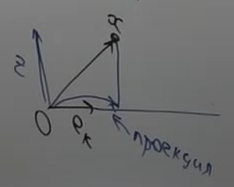
\includegraphics[width=7cm]{./assets/05-fourierreihe/projection-of-x.png}
            \end{center}
        }
    \end{enumerate}
\end{remark}

\begin{theorem}
    \textbf{о частичных суммах ряда Фурье}

    $x \in H, \{ e_n \}$ ортогональная система и $S_n = \sum_{k = 1}^n c_k (x) e_k $ - частичная сумма ряда Фурье для $x$.
    $L_n$ - линейная оболочка $\{ e_1, \ldots e_n \}$

    Тогда:
    \begin{enumerate}
        \item $S_n$ - ортогональная проекция $x$ на $L_n$, то есть $x = S_n + z$, где $z \bot L_n$
        \item $S_n$ - наилучшее приближение к $x$ в $L_n$, т.е. $||x - S_n|| = \min_{y \in L_n} ||x - y||$
        \item $||S_n|| \leqslant ||x||$
    \end{enumerate}
    
\end{theorem}

\begin{proof}
    \begin{enumerate}
        \item {
            $z = x - S_n$, надо доказать, что $z \bot L_n$, то есть $z \bot e_j$ при $j = 1, \ldots, n$

            $\left < z, e_j \right > = \left < x, e_j \right > - \left < S_n, e_j \right > = \left < x, e_j \right > - \left < \sum_{k = 1}^n c_k (x) e_k, e_j \right > = 
            \left < x, e_j \right > - c_j (x) \left < e_j, e_j \right > = 0$
        }
        \item {
            $x - \underbrace{y}_{\in L_n} = \underbrace{S_n + z - y}_{z \bot L_n} = z + (S_n - y)$
            
            Тогда $||x - y||^2 = || \underbrace{S_n - y}_{\in L_n} + \underbrace{z}_{\bot L_n} ||^2 = ||z||^2 + ||S_n - y||^2 \geqslant ||z||^2 = ||x - S_n||^2$ и равенство $\Longleftrightarrow y = S_n$
        }
        \item {
            $x = S_n + z$ и $z \bot S_n = (*)$

            Тогда $||x||^2 = || S_n + z ||^2 \underbrace{=}_{\text{т.к. } (*)} ||S_n||^2 + ||z||^2 \geqslant ||S_n||^2$
        }
    \end{enumerate}
\end{proof}

\begin{consequence}
    \textbf{Неравенство Бесселя}

    $\sum_{n = 1}^\infty |c_n (x)|^2 ||e_n||^2 \leqslant ||x||^2$
\end{consequence}

\begin{proof}
    $||x||^2 \geqslant ||S_n||^2 = \left < \sum_{k = 1}^n c_k (x)e_k, \sum_{k = 1}^n c_k (x)e_k \right > = \sum_{k  = 1}^n |c_k (x)|^2 ||e_k||^2$ и $n \to \infty$
\end{proof}

\begin{theorem}
    \textbf{Рисса-Фишера}

    $H$ - гильбертово пространство, $\{ e_n \}$ - ортогональная система в $H$ и $x \in H$. Тогда:

    \begin{enumerate}
        \item {
            Ряд Фурье $\sum_{n = 1}^\infty c_n (x) e_n$ сходится
        }
        \item {
            $x = \sum_{n = 1}^\infty c_n (x) e_n + z$, где $z \bot e_n \, \forall n$

        }
        \item {
            $x = \sum_{n = 1}^\infty c_n(x) e_n \Longleftrightarrow ||x||^2 \overset{\text{Тождество Парсеваля}}{=} \sum_{n = 1}^\infty |c_n (x)|^2 ||e_n||^2$
        }
    \end{enumerate}
\end{theorem}

\begin{proof}
    \begin{enumerate}
        \item {
            $\sum_{n = 1}^\infty c_n (x) e_n$ - сходится $\Longleftrightarrow \underbrace{\sum_{n = 1}^\infty ||c_n (x) e_n||^2}_{= \sum_{n = 1}^\infty |c_n (x)|^2 ||e_n||^2 \leqslant ||x||^2 < +\infty} < +\infty$
        }
        \item {
            $z = x - \sum_{k = 1}^\infty c_k(x)e_k$

            $\left < z, e_n \right > = \left < x, e_n \right > - \left < \sum_{k = 1}^\infty c_k (x) e_k, e_n \right > = \left < x, e_n \right > - c_n(x) \left < e_n, e_n \right > = 0$
        }
        \item {
            $x = \sum_{k = 1}^\infty c_k (x) e_k + z$, где $z \bot e_n \forall n$

            Тогда $||x||^2 = ||z||^2 + \sum_{k = 1}^\infty |c_k (x)|^2 ||e_k||^2$, то есть $z = 0 \Longleftrightarrow ||x||^2 = \sum_{k = 1}^\infty |c_k(x)|^2 ||e_k||^2$
        }
    \end{enumerate}
\end{proof}

\begin{remark}
    $\sum_{n = 1}^\infty c_n (x) e_n$ - это ортогональная проекция на $Cl \left( Lin \, \{ e_n \} \right)$, где $Lin \{ \ldots \}$ -- линейная оболочка векторов.
\end{remark}

\begin{remark}
    Если $\sum_{n = 1}^\infty |c_k|^2 ||e_k||^2 < +\infty$, то найдётся $x \in H$, для которого $\sum_{k = 1}^\infty c_k e_k$ - ряд Фурье
\end{remark}

\begin{definition}
    $\{ e_n \}$ - ортогональная система в $H$

    \begin{enumerate}
        \item {
            $\{ e_n \}$ - базис, если $\forall x \in H \, : \, x = \sum_{n = 1}^\infty c_n (x) e_n$
        }
        \item {
            $\{ e_n \}$ - полная, если из того, что $z \bot e_n \, \forall \, n \implies z = 0$
        }
        \item {
            $\{ e_n \}$ - замкнутая, если $\forall \, x \in H \, : \, ||x||^2 = \sum_{k = 1}^\infty |c_k (x)|^2 ||e_k||^2$

        }
    \end{enumerate}
\end{definition}

\begin{theorem}
    $\{ e_n \}$ ортогональная система в $H$. Следующие условия равносильны:

    \begin{enumerate}
        \item $\{ e_n \}$ - базис
        \item $\{ e_n \}$ - полная
        \item $\{ e_n \}$ - замкнутая 
        \item $\forall \, x, y \in H \, : \, \left < x, y \right > = \sum_{n = 1}^\infty c_n (x) \overline{c_n (y)} ||e_n||^2$
        \item $Cl \; Lin \; \{ e_n \} = H$
    \end{enumerate}
\end{theorem}

\begin{proof}
    \begin{enumerate}
        \item {
            $4 \implies 3$

            Берём $x = y$
        }
        \item {
            $1 \implies 4$

            $\left < x, y \right > = \left < \sum_{k = 1}^\infty c_k(x) e_k, \sum_{n = 1}^\infty c_n (y) e_n \right > = \sum_{n = 1}^\infty c_n(x) \overline{c_n(y)} ||e_n||^2$
        }
        \item {
            $3 \implies 2$

            Возьмём $z \bot e_n \, \forall n$. Тогда $||z||^2 = \sum_{n = 1}^\infty \underbrace{|c_n (z)|^2}_{= 0} ||e_n||^2 = 0 \implies z = 0$
        }
        \item {
            $2 \implies 1$

            Рисс-Фишер $\implies x = z + \sum_{k = 1}^\infty c_k (x) e_k$ и $z \bot e_n \, \forall \, n$, то есть по пункту $z=0$.
        }
        \item {
            $1 \implies 5$

            $x = \sum_{k = 1}^\infty c_k (x) e_k = \lim_{n \to +\infty} \underbrace{\sum_{k = 1}^n c_k (x) e_k}_{\in Lin \, \{ e_n \}} \implies$
            
            $\implies \lim \in Cl \, Lin \, \{ e_n \} \implies x \in Cl \, Lin \, \{ e_n \} \implies H \subset Cl \, Lin \, \{ e_n \}$ -- так как $x$ произвольный вектор из $H$.
        }
        \item {
            $5 \implies 2$

            Пусть $z \bot e_n \, \forall \, n$. Тогда $z \bot Lin \, \{ e_n \} \implies z \bot Cl \, Lin \, \{ e_n \} = H \implies z \bot z \implies z = 0$
        }
    \end{enumerate}
\end{proof}

\begin{example}
    Ортогональные системы

    \begin{enumerate}
        \item {
            Функция Радемахера $L^2 [0, 1]$

            $r_k (t) = (-1)^{[2^k t]}$, где $k = 0, 1, 2, \ldots$
            % TODO, картинка

            Это ортонормированная система, покажем это:

            $\mathds{1}_{[\frac{j}{2^k}, \frac{j + 1}{2^k}]} (t) r_n (t) = 0$ и $\int_{0}^1 r_i (t) r_j (t) \, dt = 0$

            Она не полная: $r_1r_2 \bot r_n \, \forall \, n$
        }
        \item {
            Функция Уолша. Пространство $L^2 [0, 1]$

            $A \subset \mathbb{N}$ и $\#A < +\infty$. Пусть $w_A (t) = \prod\limits_{k \in A} r_k (t)$

            Это ортонормированная система:

            $\left < w_A, w_B \right > = \left < w_{A \setminus B} , w_{B \setminus A} \right > = 
            \int_0^1 \prod_{i \in } r_i (t) \, dt = 0$

            Это полная система $Cl \, Lin \, w_A = L^2 [0, 1]$

            $Lin_{A \subset \{ 0, 1, \ldots, n \}} \,  w_A = Lin_{j = 0, 1, \ldots, 2^n - 1} \, \mathds{1}_{[\frac{j}{2^n}, \frac{j + 1}{2^n}]}$. 
            Тогда $Lin \, w_A = Lin \, \mathds{1}_{(\frac{j}{2^n}, \frac{j + 1}{2^n}]}$
        }
        \item {
            Функции Хаара. Пространство $L^2 [0, 1]$

            \begin{enumerate}
                \item {
                    $h_0 (t) \equiv 1$
                }
                \item {
                    $h_1 (t) = \begin{cases}
                        +1, & \text{на $[0, \frac{1}{2})$} \\
                        -1, & \text{на $[\frac{1}{2}, 1)$}
                    \end{cases}$
                }
                \item {
                    $h_2 (t) = \begin{cases}
                        +1, & \text{на $[0, \frac{1}{4})$} \\
                        -1, & \text{на $[\frac{1}{4}, \frac{1}{2})$}
                    \end{cases}$
                }
                \item {
                    $h_3 (t) = \begin{cases}
                        +1, & \text{на $[\frac{1}{2} \frac{3}{4})$} \\
                        -1, & \text{на $[\frac{3}{4}, 1)$}
                    \end{cases}$
                }
                \item {
                    $\ldots$    
                }
            \end{enumerate}
        }
    \end{enumerate}

    Это ортогональная система и полная система

    $Lin \, \{ h_0, h_1, \ldots h_{2n} \} = Lin \, \mathds{1}_{[\frac{j}{2^n}, \frac{j + 1}{2^n})}$
\end{example}

\begin{remark}
    \textbf{Ортогонализация Грамма-Шмидта}

    $\{ x_1, x_2, \ldots \}$ линейно независимые вектора.

    Тогда существуют $\{ e_1, e_2, \ldots  \}$ - ортонормированная система, т.ч.:
    $Lin \, \{ e_1, \ldots \} = Lin \, \{ x_1, x_2, \ldots \}$

    Если $f_1, f_2, \ldots$ тоже ортонормированная система с тем же свойством, то 
    $f_k = \lambda_k e_k$, где $|\lambda_k| = 1$
    
    \begin{remark}
        Пусть $w \, : \, \mathbb{R} \rightarrow [0, +\infty)$ измеримая,
        т.ч. $t^n w(t)$ - суммируемая на $\mathbb{R} \, \forall \, n$. Определим меру $\mu A = \int_A w \, d\lambda$ и пространство будет $L^2 (\mathbb{R}, \mu)$

        Если $f \bot g$ в таком пространстве, то они ортогональны с весом $w$

        Рассмотрим последовательность мономов $1, t, t^2, \ldots \in L^2 (\mathbb{R}, \mu)$, они линейно независимы.

        Тогда мы можем прокрутить ортогонализацию Грамма-Шмидта на этой последовательности мономов. Получим последовательность многочленов $p_0, p_1, \ldots$.
        Мы понимаем, что $\left < p_i, p_j \right > = 0 \, \forall \, i \neq j$. А ещё $\deg p_n = n$ - по индукции.

        Получившиеся многочлены называют ортогональными многочленами с весом $w$.

        \begin{example}
            Ортогональные многочлены.

            \begin{enumerate}
                \item {
                    Многочлены Лежандра. Пространство $L^2 (-1, 1)$

                    $P_n (t) = \frac{1}{2^n \cdot n!} ((t^2 - 1)^n)^{(n)}$, считаем, что $n > k$:

                    $\left < P_k, P_n \right > = \underbrace{\frac{1}{2^n \cdot n!} \cdot \frac{1}{2^k \cdot k!}}_{=C} \int_{-1}^1 ((t^2 - 1)^k)^{(k)} ((t^2 - 1)^n)^{(n)} \, dt =$
                    
                    $= C \left( ((t^2 - 1)^k)^{(k)} \cdot ((t^2 - 1)^n)^{(n - 1)} \bigg |_{-1}^1 - \int_{-1}^1 ((t^2 - 1)^k)^{(k + 1)} ((t^2 - 1)^n)^{(n - 1)} \, dt \right) = \ldots$
                    
                    $= \pm C \int_{-1}^1 \underbrace{((t^2 - 1)^k)^{(2k + 1)}}_{=0} ((t^2 - 1)^n)^{(n - k - 1)} \, dt = 0$
                }
                \item {
                    Многочлены Чебышёва первого рода. Пространство $L^2 ((-1, 1), w(t) = \frac{1}{\sqrt{1 - t^2}})$

                    $T_n (t) = \cos (n \arccos t)$ - оказывается, что это многочлен. Проверить можно по индукции.

                    $\left < T_k, T_n \right > = \int_{-1}^1 \cos (k \arccos t) \cdot \cos (n \arccos t) \cdot \frac{dt}{\sqrt{1 - t^2}} = (*)$

                    Пусть $x = \arccos t$. Тогда $dx = \frac{1}{\sqrt{1 - t^2}}$

                    $(*) = \int_0^\pi \cos (kx) \cos (nx) \, dx = 0$
                }
                \item {
                    Многочлены Чебышёва второго рода. Пространство $L^2 ((-1, 1), w(t) = \sqrt{1 - t^2})$

                    $U_n (t) = \frac{\sin ((n + 1) \arccos t)}{\sqrt{1 - t^2}}$

                    $\left < U_k, U_n \right > = \int_{-1}^1 \frac{\sin ((k + 1) \arccos t)}{\sqrt{1 - t^2}} \cdot \frac{\sin ((n + 1) \arccos t)}{\sqrt{1 - t^2}} \cdot \sqrt{1 - t^2} \, dt = \int_0^\pi \sin ((n + 1)x) \sin ((k + 1)x) \, dx = 0$ - такая же замена.
                }
                \item {
                    Многочлены Лагерра. Пространство $L^2 ((0, +\infty), w(t) = e^{-t})$

                    $L_n (t) = \frac{1}{n!} e^t (t^n e^{-t})^{(n)}$

                    Ортогональность проверяется также, как в Лежандре - интегрированием по частям.
                }
                \item {
                    Многочлены Эрмита. Пространство $L^2 (\mathbb{R}, w(t) = e^{-t^2})$

                    $H_n (t) = e^{t^2} (e^{-t^2})^{(n)}$

                    Ортогональность проверяется опять интегрированием по частям.
                }
            \end{enumerate}
        \end{example}
    \end{remark}
\end{remark}

\begin{definition}
    $(X, \rho)$ - метрическое пространство, $A \subset X$, и есть точка $x \in X$. Назовём расстоянием от $x$ до $A$ (или наилучшим приближением к $x$ в множестве $A$):
    
    $d(x, A) = \inf_{y \in A} \rho (x, y)$ 
\end{definition}

\begin{definition}
    Элемент $y^{*} \in A$ элемент наилучшего приближения, если $\rho (x, y^*) = d(x, A)$
\end{definition}

\begin{theorem}
    \textbf{о существовании наилучшего приближения в гильбертовом пространстве}

    $H$ - гильбертово пространство, $A \subset H$ - выпуклое и замкнутое и $x \in H$.

    Тогда в $A$ существует единственный элемент наилучшего приближения.
\end{theorem}

\begin{lemma}
    $||x + y||^2 + ||x - y||^2 = 2||x||^2 + 2||y||^2 $
\end{lemma}

\begin{proof}
    Теоремы.

    Пусть $d = d(x, A)$ -- оно конечно. Возьмём $y, z \in A$, тогда $\frac{y + z}{2} \in A$ из выпуклости.

    \begin{center}
        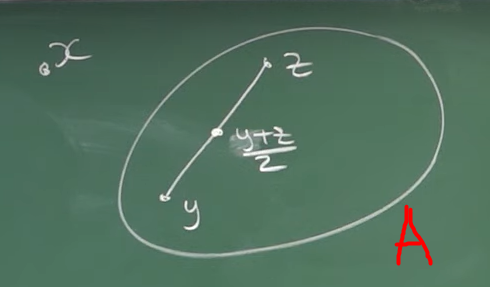
\includegraphics[width=8cm]{assets/05-fourierreihe/existance-of-the-best-approximation.png}
    \end{center}
    
    $\underbrace{|| 2 \left(x - \frac{y + z}{2}\right) ||^2}_{= 4 || x - \frac{y + z}{2} || \geqslant 4d^2} + ||y - z||^2 = 2 ||x - y||^2 + 2||x - z||^2 \geqslant 4d^2$ -- подставили в лемму $x - y$ и $x - z$.

    Отсюда $||y-z||^2 = 2 ||x - y||^2 + 2 ||x - z||^2 - 4 || x - \frac{y + z}{2}|| \leqslant 2 ||x - y||^2 + 2||x - z||^2 - 4d^2$

    \begin{enumerate}
        \item {
            \textbf{Единственность}:

            Если $||x - y||^2 = d$ и $||x - z||^2 = d$, то $||y - z||^2 \leqslant 0 \implies y = z$
        }
        \item {
            \textbf{Существование}:

            Возьмём $y_n$, т.ч. $||x - y_n|| \rightarrow d$, то есть $|| x - y_n ||^2 < d^2 + \varepsilon$.
            
            Тогда $||y_n - y_m||^2 \leqslant 2 ||x - y_n||^2 + 2||x - y_m||^2 - 4d^2 < 4\varepsilon$, значит это фундаментальная последовательность и у нее есть предел $y^* \in A$, поскольку $A$ -- замкнуто.
            
            $||x - y^*|| = \lim_{n \to \infty} ||x - y_n|| = d$.
        }
    \end{enumerate}
\end{proof}

\begin{theorem}
    \textbf{теорема о проекции}

    $H$ - гильбертово пространство, $L$ - замкнутое подпространство $H$

    Тогда $\forall \, x \in H \, : \, \exists \, y \in L \, : \, \underbrace{x - y}_{=z} \bot L$ и 
    такой $y$ единственный.
\end{theorem}

\begin{proof}
    \textit{Единственность}:

    $x = y + z = y_1 + z_1$, $y, y_1 \in L$ и $z, z_1 \bot L \implies \underbrace{y - y_1}_{\in L} = \underbrace{z_1 - z}_{\bot L} \implies z_1 - z \bot y - y_1 = z_1 - z \implies z = z_1 \implies y = y_1$

    \textit{Существование}:

    Пусть $y$ - элемент наилучшего приближения к $x$ в $L$

    $z = x - y, l \in L, \lambda \in \mathbb{C}$

    Мы знаем, что $\underbrace{|| x - y ||^2}_{= |||z||^2} \leqslant \underbrace{|| x - (y - \lambda l) ||^2}_{||z + \lambda l||^2} \implies \left < z, z \right > \leqslant \left < z, z \right > + \left < z, \lambda l \right > + \left < \lambda l, z \right > + \left < \lambda l, \lambda l \right >$

    $|\lambda|^2 \left < l, l \right > + \lambda \left < l, z \right > + \overline{\lambda} \left < z, l \right > \geqslant 0$

    $|\lambda|^2 \left < l, l \right > + 2 \Re (\lambda \left < l, z \right >) \geqslant 0$ при всех $\lambda \in \mathbb{C}$

    Возьмём $\lambda = -\frac{\left < z, l \right >}{||l||^2}$

    Подставляем: $\frac{|\left < z, l \right >|^2}{||l||^2} - 2\Re \left( \frac{|\left < z, l \right >|^2}{||l||^2} \right) \geq 0 \implies \frac{|\left < z, l \right >|^2}{||l||^2} \geq 2 \cdot \frac{|\left < z, l \right >|^2}{||l||^2} \implies - \frac{|\left <z, l \right >|^2}{||l||^2} \geq 0 \implies z \bot l$
\end{proof}

\begin{definition}
    Этот $y$ называется ортогональной проекцией $x$ на $L$
    
    То есть получилось отображение $P_L \, : \, H \to L$ - оператор ортогонального проецирования
\end{definition}

\begin{definition}
    Ортогональное дополнение. Пусть $L$ замкнутое подпространство $H$. Тогда $L^\bot = \{ x \in H \, : \, x \bot L \}$ - замкнутое подпространство $H$
\end{definition}

\begin{properties}
    \begin{enumerate}
        \item { $P_L$ - линейный оператор
            \begin{proof}
                $y_1 = P_L x_1$ и $y_2 = P_L x_2 \implies x_1 - y_1 \bot L$ и $x_2 - y_2 \bot L$

                Тогда $(\alpha_1 x_1 + \alpha_2 x_2) - (\alpha_1 y_1 + \alpha_2 x_2) \bot L \implies \alpha_1 y_1 + \alpha_2 y_2 = P_L (\alpha_1 x_1 + \alpha_2 x_2)$
            \end{proof}
        }
        \item {
            Если $L \neq \{ 0 \}$, то $||P_L|| = 1$

            \begin{proof}
                $y = P_L x \implies x = y + z$, где $y \in L, z \in L \implies y \bot z$

                $||x||^2 = ||y||^2 + ||z||^2 \geqslant ||y||^2 \implies ||x|| \geqslant ||P_L x|| \implies ||P_L|| \leqslant 1$

                Если $L \neq \{ 0 \}$, то возьмём в $L$ единичный вектор и он переходит в себя
            \end{proof}
        }
        \item {
            $P_{L^\bot} = Id - P_L$

            \begin{proof}
                $x = y + z$, где $y \in L, z \in L \implies Z \in L^\bot$ и $y \bot L^\bot$

                Тогда $y = P_L x$ и $z = P_{L^\bot} x \implies x = P_{L} x + P_{L^\bot} x$
            \end{proof}
        }
        \item {
            $(L^\bot)^\bot = L$  

            \begin{proof}
                $P_{(L^\bot)^\bot} = Id - P_{L^\bot} = Id - (Id - P_L) = P_L$

                $(L^\bot)^\bot = P_{(L^\bot)^\bot} (H) = P_L (H) = L$
            \end{proof}
        }
    \end{enumerate}
\end{properties}

\begin{definition}
    $(X, \rho)$ - метрическое пространство.

    $X$ - сепарабельное, если существует счётное множество $A \subset X$, т.ч. $Cl \, A = X$
\end{definition}

\begin{example}
    \begin{enumerate}
        \item {
            $\mathbb{R}^d$ и $A = \mathbb{Q}^d$
        }
        \item {
            $p < +\infty$, $L^p (\mathbb{R}^d, \lambda_d)$

            $A = \{ \text{линейные комбинации с $\mathbb{Q}$ коэффициентами $\mathds{1}_B$, где $B$ - ячейка с $\mathbb{Q}$ коорд. вершин} \} $

            Для $p = +\infty$, здесь $L^\infty (\mathbb{R}^d, \lambda_d)$ не сепарабельно
        }
    \end{enumerate}
\end{example}

\begin{theorem}
    В сепарабельном гильбертовом пространстве обязательно существует базис
\end{theorem}

\begin{proof}
    $\{ x_n \}$ - счётное множество, т.ч. $Cl \, \{ x_n \} = H$

    $x_1, x_2, \ldots x_k$, $x_k$ оставляем, только если он линейно независим от $x_1, \ldots, x_{k - 1}$, иначе выкидываем

    Пусть $y_1, y_2, \ldots$ - уже прореженные $x_1, x_2, \ldots$

    Тогда $Lin \, \{ y_n \} = Lin \, \{ x_n \} \implies Cl \, Lin \, \{ y_n \} = Cl \, Lin \, \{ x_n \} = H$

    $y_1, y_2, \ldots$ - линейно независимая система, запустим ортогонализацию Грамма-Шмидта, получим $e_1, e_2, \ldots$.
    Мы знаем, что $Lin \, \{ e_i \}_{i = 1}^n = Lin \, \{ y_i \}_{i = 1}^n \implies Lin \, \{ e_n \} = Lin \, \{ y_n \} = Lin \, \{ x_n \} \implies Cl \, Lin \, \{e_n \} = H$, значит это базис
\end{proof}

\begin{theorem}
    Бесконечномерное сепарабельное гильбертово пространство $H$ изометрично $l^2$

    То есть существует линейный оператор $T \, : \, H \to l^2$, т.ч. $T$ - биекция и $\forall \, x, y \in H \, : \, \left < x, y \right >_H = \left < T_x, T_y \right >_{l^2}$
\end{theorem}

\begin{proof}
    Возьмём базис $e_1, e_2, \ldots$, он счётный и отнормируем.
    
    Тогда $x \rightarrow (\left < x, e_1 \right >, \left < x, e_2 \right >, \ldots)$.
    
    Хотим показать, что это то, что надо.

    \begin{enumerate}
        \item {
            Попадание в $l^2$

            $\sum\limits_{k = 1}^\infty |\left < x, e_k \right >|^2 \overset{\text{неравенство Бесселя}}{\leqslant} ||x||^2 < +\infty$
        }
        \item {
            Сохранение скалярного произведения

            $\left < x, y \right >_H = \sum\limits_{k = 1}^\infty \left < x, e_k \right > \overline{\left < y, e_k \right >}$ - была такая теорема
         }
    \end{enumerate}
\end{proof}

\Subsection{Тригонометрические ряды Фурье}

\begin{definition}
    $\frac{a_0}{2} + \sum_{k = 1}^n (a_k \cos (kx) + b_k \sin (kx))$ - тригонометрический многочлен

    А если $|a_n| + |b_n| \neq 0$, то тригонометрический многочлен степени $n$
\end{definition}

\begin{definition}
    $\frac{a_0}{2} + \sum_{k=1}^\infty (a_k \cos (kx) + b_k \sin (kx))$ - тригонометрический ряд
\end{definition}

\textbf{Комплексная форма тригонометричсекого многочлена}

$\cos (kx) = \frac{e^{ikx} + e^{-ikx}}{2}$ и $\sin (kx) = \frac{e^{ikx} - e^{-ikx}}{2i}$

$T_n (x) = \frac{a_0}{2} + \sum_{k = 1}^n \left ( e^{ikx} \cdot \underbrace{\frac{a_k - ib_k}{2}}_{=c_k} + e^{-ikx} \cdot \underbrace{\frac{a_k + ib_k}{2}}_{=c_{-k}} \right ) = \sum_{k = -n}^n c_k e^{ikx}$

\textbf{Комплексная форма тригонометрического ряда}

$\sum_{k = -n}^n c_k e^{ikx} \rightarrow \sum_{k = -\infty}^{+\infty} c_k e^{ikx}$

\begin{theorem}
    Если тригонометрический ряд сходится в пространстве $L^1 [-\pi, \pi]$ к функции $f$, то
    $a_k = \frac{1}{\pi} \int_{-\pi}^\pi f(x) \cos (kx) \, dx$, $b_k = \frac{1}{\pi} \int_{-\pi}^\pi f(x) \sin (kx) \, dx$ и 
    $c_k = \frac{1}{2\pi} \int_{-\pi}^\pi f(x) e^{-ikx} \, dx$
\end{theorem}

\begin{proof}

    $T_n (x) = \frac{a_0}{2} + \sum_{k = 1}^n (a_k \cos (kx) + b_k \sin (kx))$ -- частичная сумма ряда.

    Пусть $n \geq m$:

    $|\underbrace{\int_{-\pi}^{\pi} T_n(x) \cos{(m x)} dx}_{= a_m \cdot \pi \text{, т.к. везде будут нули, кроме $m$-ого элемента}} - \int_{-\pi}^{\pi} f(x) \cos{(m x)} dx| =$
    
    $= |\int_{-\pi}^{\pi} \left(T_n(x) - f(x)\right) \cos{(m x)} dx | \leq \int_{-\pi}^{\pi} |T_n(x) - f(x)| dx = || T_n - f ||_1 \to_{n \to \infty} 0$

    Тогда доказали, что хотели, так как $\frac{1}{\pi} \int_{-\pi}^{\pi} f(x) \cos{(mx)} dx$ стремится к $a_m$ (по аналогии для $b_m$ и $c_m$).

    % $||T_n - f ||_{L^1 [-\pi, \pi]} = \int_{-\pi}^\pi |T_n(x) - f(x)| \, dx \rightarrow 0$

    % $\int_{-\pi}^\pi T_n(x) \cos (kx) \, dx = \frac{a_0}{2} \int_{-\pi}^\pi \cos (kx) \, dx + \sum_{j = 1}^n a_k \int_{-\pi}^\pi \cos (jx) \cos (kx) \, dx + \sum_{j = 1}^n b_j \int_{-\pi}^\pi \sin (jx) \cos (kx) \, dx = a_k \pi$
\end{proof}

\begin{definition}
    Пусть $f \in L^1 [-\pi, \pi]$, тогда
    
    $a_k (f) = \frac{1}{\pi} \int_{-\pi}^\pi f(x) \cos (kx) \, dx$, $b_k (f) = \frac{1}{\pi} \int_{-\pi}^\pi f(x) \sin (kx) \, dx$ и 
    $c_k(f) = \frac{1}{2\pi} \int_{-\pi}^\pi f(x) e^{-ikx} \, dx$ - коэффициенты Фурье для функции $f$, а соответствующий ряд называется рядом Фурье
\end{definition}

\begin{remark}
    Если $f$ - сумма сх-ся в $L^1 [-\pi, \pi]$ тригонометрического ряда, то это её ряд Фурье

    Вопрос, когда $f (x) = \frac{a_0 (f)}{2} + \sum_{k = 1}^\infty (a_k (f) \cos (kx) + b_k (f) \sin (kx))$

    \begin{enumerate}
        \item {
            Дюбуа-Реймон показал, что $\exists \, f$ непрерывная $2\pi$ периодическая, т.ч. её ряд Фурье расходится в некоторой точке
        }
        \item {
            Лебег показал, что $\exists \, f$ непрерывная $2\pi$ периодическая, т.ч. ряд Фурье сходится во всех точках, но нет равномерной сходиомсти
        }
        \item {
            Колмогоров показал, что $\exists \, f \in L^1 [-\pi, \pi]$, т.ч. её ряд Фурье расходится во всех точках
        }
        \item {
            Карлесон показал, что $\forall \, f \in L^2 [-\pi, \pi]$ ряд Фурье сходится почти везде
        }
        \item {
            Рисс показал, что $1 < p < +\infty \, \forall \, f \in L^p [-\pi, \pi]$ ряд сходится к $f$ в $L^p$
        }
    \end{enumerate}

    $C_{2\pi}$ - непрерывные $2\pi$ периодичные функции

    $A_k (f, x) = \begin{cases}
        \frac{a_0(f)}{2} \text{, если $k = 0$} \\
        a_k (f) \cos (kx) + b_k (f) \sin (kx) \text{, иначе}
    \end{cases}$
\end{remark}

\textbf{Дискретное преобразование Фурье}

$x_0, x_1, \ldots, x_{N - 1} \rightarrow a_0, a_1, \ldots, a_{N - 1}$

$a_k = \sum\limits_{n = 0}^{N - 1} x_n e^{-\frac{2\pi i}{N} kn}$

$x_n = \frac{1}{n} \sum\limits_{k = 0}^{N - 1} a_k e^{\frac{2\pi i}{N} kn}$

% TODO, Картинка

$f(t) = x_n$ при $\frac{2\pi}{N}n < t \leqslant \frac{2\pi}{N} (n + 1)$. Тогда $c_k (f) = \frac{1}{\pi} \int_0^{2\pi} f(t) e^{-itk}\, dt = \\
\frac{1}{2\pi} \sum\limits_{n = 0}^{N - 1} x_n \underbrace{\int_{\frac{2\pi}{N} n}^{\frac{2\pi}{n} (n + 1)} e^{-itk} \, dt}_{=\frac{e^{-itk}}{-ik} \bigg |_{\frac{2\pi}{n} n}^{\frac{2\pi}{n} (n + 1)} = \frac{i}{k} e^{-\frac{2\pi}{N}kn} (1 - e^{-ik\frac{2\pi}{N}})} = 
\frac{i}{2\pi} \frac{1 - e^{-ik\frac{2\pi}{N}}}{k} \underbrace{\sum_{n = 0}^{N - 1} x_n e^{-\frac{2\pi}{N} kn}}_{= a_k}$ 

\begin{lemma}
    \textbf{Римана-Лебега}

    Пусть $f \in L^1 (E)$, тогда $\int_E f(t) e^{-i t \lambda} \, dt$, $\int_E f(t) \cos (\lambda t) \, dt$, $\int_E f(t) \sin (\lambda t) \, dt \rightarrow 0$
\end{lemma}

\begin{proof}
    Продолжим нулём фукнцию на $\mathbb{R} \implies f \in L^1 (\mathbb{R})$

    $\int_{\mathbb{R}} f(t) e^{-i t \lambda} \, dt = \int_{\mathbb{R}} f(u + h) e^{iu\lambda} \, du \cdot  e^{ih\lambda} = \overset{h = \frac{\pi}{\lambda}}{=} - \int_{\mathbb{R}} f(u + \frac{\pi}{\lambda}) e^{iu\lambda} \, du$

    Посмотрим на 2 таких интеграла: $2 \int_{\mathbb{R}} f(t) e^{-i \lambda t} \, dt = \int_{\mathbb{R}} f(t) e^{-i \lambda t} \, dt - \int_{\mathbb{R}} f(u + \frac{\pi}{\lambda}) e^{-i\lambda u} \, du = \int_{\mathbb{R}} (f(t) - f(t + \frac{\pi}{\lambda})) e^{-i \lambda t} \, dt $

    $2 \left | \int_{\mathbb{R}} f(t) e^{-i \lambda t} \, dt \right | \leqslant \int_{\mathbb{R}} \left | f(t) - f(t + \frac{\pi}{\lambda}) \right | \, dt = || f - f_h ||_1 \rightarrow 0$, по теореме о непрерывности сдвига

    Для синуса и косинуса всё аналогично
\end{proof}

\begin{consequence}
    Если $f \in L^1 (-\pi, \pi)$, то $a_k (f), b_k (f), c_k (f) \overset{|k| \to \infty}{\rightarrow} 0$
\end{consequence}

\begin{definition}
    Модуль непрерывности $w_f (\delta) = \sup\limits_{|x - y| \leqslant \delta} |f(x) - f(y)|$

    \begin{remark}
        $f$ равномерно непрерывна $\Longleftrightarrow \lim\limits_{\delta \to 0+} w_f (\delta) = 0$
    \end{remark}
\end{definition}

\begin{definition}
    Липшицева функция порядка $\alpha$ с константой $M$. Обозначение $Lip_\alpha M$

    $\forall \, x, y, \, : \, |f(x) - f(y)| \leqslant M \cdot |x - y|^\alpha$, $\alpha \in (0, 1]$
\end{definition}

\begin{definition}
    $Lip_\alpha = \bigcup\limits_{M > 0} Lip_\alpha M$
\end{definition}

\begin{remark}
    Если $f \in Lip_\alpha M$, то $w_f (\delta) \leqslant M \delta^\alpha$
\end{remark}

$C_{2\pi}$ - непрерывные $2\pi$-периодические функции

\begin{theorem}
    Если $f \in C_{2\pi}$, то $|a_k (f)|, |b_k (f)|, 2|c_k (f)| \leqslant w_f (\frac{\pi}{|k|})$
\end{theorem}

\begin{proof}
    $2\pi 2c_k (f) = 2 \int_{-\pi}^\pi f(t) e^{-ikt} \, dt = \int_{-\pi}^\pi f(t) e^{-ikt} \, dt + \int_{-\pi - \frac{-\pi}{k}}^{\pi - \frac{\pi}{k}} f(u + \frac{\pi}{k}) e^{-iku} \, du \cdot e^{-\pi i} = 
    \int_{-\pi}^\pi f(t) e^{-ikt} \, dt - \int_{-\pi}^{\pi} f(u + \frac{\pi}{k}) e^{-iku} \, du = \int_{-\pi}^\pi (f(t) - f(t + \frac{\pi}{k})) e^{-ikt} \, dt$

    $4\pi |c_k (f)| \leqslant \int_{-\pi}^\pi |f(t) - f(t + \frac{\pi}{k})| \, dt \leqslant 2\pi w_f (\frac{\pi}{|k|})$

    Для остальных аналогично
\end{proof}

\begin{consequence}
    Если $f \in Lip_\alpha M$ и $2\pi$ периодическая, то
    $|a_k (f)|, |b_k(f) |, | c_k(f) | \leqslant M \left (\frac{\pi}{|k|} \right )^\alpha$
\end{consequence}

\begin{lemma}
    Пусть $f \in C_{2\pi}^1$

    Тогда $a_n (f') = n b_n (f)$, $b_n (f') = -n a_n (f)$ и $c_n (f') = in c_n (f)$
\end{lemma}

\begin{proof}
    $c_n (f') = \frac{1}{2\pi} \int_{-\pi}^\pi f'(t) e^{-int} \, dt = \frac{1}{2\pi} f(t) e^{-int} \bigg |_{t = -\pi}^{t = \pi} = -\frac{1}{2\pi} \int_{-\pi}^\pi f (t) (-ine^{-int}) \, dt = 
    in \frac{1}{2\pi} \int_{-\pi}^\pi f(t) e^{-int} \, dt = in c_n (f)$

    Остальные аналогично
\end{proof}

\begin{consequence}
    Если $f \in C_{2\pi}^r$ и $f^{(r)} \in Lip_{\alpha} M$, то $|a_n(f)|, |b_n (f)|, |c_n (f)| \leqslant M \frac{\pi^\alpha}{|n|^{r + 2}}$
\end{consequence}

\begin{proof}
    $|c_n (f)| = \frac{|c_n (f^{(r)})|}{n^r}$
\end{proof}

\begin{definition}
    Ядро Дирихле

    $D_n (t) = \frac{1}{2} + \sum_{k = 1}^n \cos (kt)$
\end{definition}

\begin{properties}
    \begin{enumerate}
        \item $D_n$ непрерывна и $2\pi$ периодична, чётная
        \item $D_n (0) = n + \frac{1}{2}$
        \item {
            $D_n (t) = \frac{\sin (n + \frac{1}{2})t}{2\sin \frac{t}{2}}$, при $t \neq 2\pi m$

            \begin{proof}
                Индукция по $n$, база $n = 0$ верна

                Переход $n - 1 \to n$. $D_{n} (t) = D_{n - 1} (t) + \cos (nt) = \frac{\sin (n - \frac{1}{2})t}{2\sin \frac{t}{2}} + \cos (nt) = \frac{\sin (n - \frac{1}{2})t + 2\cos (nt) \sin \frac{t}{2}}{2\sin \frac{t}{2}} = \frac{\sin (n + \frac{1}{2})t}{2\sin \frac{t}{2}}$
            \end{proof}
        }
        \item $\int_{-\pi}^\pi D_n (t) \, dt = \pi$ и $\int_0^\pi D_n (t) = \frac{\pi}{2}$
    \end{enumerate}
\end{properties}

\begin{lemma}
    Пусть $f \in L^1 [-\pi, \pi]$ - суммируемая, $S_n (f, x)$ - частичная сумма ряда Фурье в точке $x$

    Тогда $S_n (f, x) = \frac{1}{\pi} \int_{-\pi}^\pi f(x \pm t) D_n (t) \, dt = \frac{1}{\pi} \int_0^\pi (f(x + t) + f(x - t)) D_n (t) \, dt$
\end{lemma}

\textbf{Напоминание}

$A_k (f, x) = 
\begin{cases}
    \frac{a_0 (f)}{2}, & \text{при $k = 0$} \\
    a_k (f) \cos (kx) + b_k (f) \sin (kx), & \text{при $k > 0$}
\end{cases}$

$A_k (f) = \frac{1}{\pi} \int_{-\pi}^\pi f(x - t) \cos (kt) \, dt$, $A_0 (f) = \frac{1}{2\pi} \int_{-\pi}^\pi f(x - t) \, dt$

\begin{proof}
    леммы

    $S_n (f, x) = \sum_{k = 0}^n A_k (f, x) = \frac{1}{2\pi} \int_{-\pi}^\pi f(x - t) \, dt +  \frac{1}{\pi} \sum_{k = 1}^{n} \int_{-\pi}^\pi f(x - t) \cos kt \, dt = 
    \frac{1}{\pi} \int_{-\pi}^\pi f(x - t) D_n (t) \, dt = \frac{1}{\pi} \int_{-\pi}^\pi f(x + u) D_n (u) (-1) \, du$
\end{proof}

\begin{consequence}
    Пусть $f \in L^1 [-\pi, \pi]$, $S_n (f, x)$ - частичная сумма ряда Фурье

    Тогда $S_n (f, x) = \frac{1}{\pi} \int_0^\delta (f(x + t) + f(x - t)) D_n (t) \, dt + o(1)$ при $n \to \infty$
\end{consequence}

\begin{proof}
    $S_n (f, x) = \frac{1}{\pi} \int_{-\pi}^\pi (f(x + t) + f(x - t)) D_n (t) \,  dt = \frac{1}{\pi} \left( \int_{0}^\delta + \int_\delta^\pi \right)$

    Надо понять, что $\int_{\delta}^\pi (f(x + t) + f(x - t)) D_n (t) \,  dt \rightarrow 0$

    $\int_{\delta}^\pi (f(x + t) + f(x - t)) D_n (t) \,  dt = \int_\delta^\pi \frac{f(x + t) + f(x - t)}{2 \sin \frac{t}{2}} \sin (n + \frac{1}{2}) t \, dt \overset{\text{Риман-Лебег}}{\rightarrow} 0$, потому что суммируема на $[\delta, \pi]$
\end{proof}

\begin{consequence}
    Принцип локализации

    $f, g \in L^1 [-\pi, \pi]$, $2\pi$ периодические

    $x \in [-\pi, \pi]$ и $f = g$ на $(x - \delta, x + \delta)$, тогда ряды Фурье для $f$ и $g$, выписанные в точке $x$ ведут себя одинаково (либо оба сходятся, либо оба расходятся)

    И если они сходящиеся, то у них одинаковая сумма, более того $S_n (f, x) - S_n (g, x) \overset{n \to +\infty}{\rightarrow} 0$
\end{consequence}

\begin{proof}
    $S_n (f, x) - S_n (g, x) = \frac{1}{\pi} \int_0^\delta (f(x + t) + f(x - t)) D_n (t) \, dt - \frac{1}{\pi} \int_0^\delta (g(x + t) + g(x - t)) D_n (t) \, dt + o(1)$, подынтегральные функции в окрестности совпадают, значит останется только $o(1)$
\end{proof}

\textbf{Обозначение. } $f(a \pm 0) = \lim\limits_{x \to a\pm} f(x)$

$f_+' (a) = \lim\limits_{h \to 0+} \frac{f(a + h) - f(a + 0)}{h}$. Если функция непрерывна в точке $a$, то такое определение совпадает с тем, что было раньше

$f_-' (a) = \lim\limits_{h \to 0+} \frac{f(a - h) - f(a - 0)}{-h}$

\begin{definition}
    $a$ - регулярная точка для $f$, если $f(a) = \frac{f(a + 0) + f(a - 0)}{2}$
\end{definition}

\begin{lemma}
    $f \in L^1 [-\pi, \pi]$, тогда $\int_0^\delta \frac{|f(t)|}{t} \, dt$ и $\int_0^\pi \frac{|f(t)|}{2\sin \frac{t}{2}} \, dt$ ведут себя одинаково, 
    если $0 < \delta < \pi$
\end{lemma}

\begin{proof}
    $\int_0^\pi \frac{|f(t)|}{2\sin \frac{t}{2}} \, dt = \int_0^\delta + \underbrace{\int_\delta^\pi}_{\leqslant \frac{1}{2\sin \frac{\delta}{2}} \int_\delta^\pi |f(t)| \, dt < +\infty } $

    Смотрим на $[0, \delta]$. $\frac{|f(t)|}{t} \leqslant \frac{|f(t)|}{2 \sin \frac{t}{2}} \leqslant \frac{|f(t)|}{t \cdot \frac{2}{\pi}}$ (из $u \frac{2}{\pi} \leqslant \sin u \leqslant i$)
\end{proof}

\textbf{Обозначение. }  $f_x^* (t) = f(x + t) + f(x - t) - f(x + 0) - f(x - 0) \overset{\text{Если $x$ - точка регулярности}}{=} f(x + t) + f(x - t) - 2f(x)$

\begin{theorem}
    \textbf{Признак Дини}

    $f \in L^{1} [-\pi, \pi], x \in [-\pi, \pi]$ - точка непрерывности или разрыва первого рода. $0 < \delta < \pi$. Если $\int\limits_0^\delta \frac{|f_x^* (t)|}{t} \, dt < +\infty$, то ряд Фурье 
    функции $f$ в точке $x$ сходится к $\frac{f(x + 0) + f(x - 0)}{2}$
\end{theorem}

\begin{proof}
    $S_n (x) = \int\limits_0^\pi (f(x + t) + f(x - t)) D_n (t) \, dt$. Ещё мы знаем, что $\int\limits_0^\pi D_n (t) \, dt = \frac{1}{2}$

    $S_n(x) - \frac{f(x + 0) + f(x - 0)}{2} = \frac{1}{\pi} \int_0^\pi f_x^* (t) D_n (t) \, dt $

    Нужно доказать, что $\int_0^\pi f_x^* (t) D_n (t) \, dt \rightarrow 0$

    $f_x^* (t) \in L^1 [-\pi, \pi]$, т.к. $|f_x^* (t)| \leqslant |f(x + t)| + |f(x - t)| + |f(x + 0)| + |f(x - 0)|$

    $D_n(t) = \frac{\sin ((n + \frac{1}{2})t)}{2\sin \frac{t}{2}}$. Значит нужно понять про $\int_0^\pi \frac{|f_x^* (t)|}{2 \sin \frac{t}{2}} \sin ((n + \frac{1}{2})t) \, dt \overset{\text{Риман-Лебег, если (*)}}{\rightarrow} 0$

    $(*) \, : \, \int_0^\pi \frac{|f_x^* (t)|}{2 \sin \frac{t}{2}} \, dt < +\infty \overset{\text{лемма}}{\Longleftrightarrow} \int_0^\delta \frac{|f_x^* (t)|}{t} \, dt < +\infty$ - а это верно из условия 
\end{proof}

\begin{consequence}
    \begin{enumerate}
        \item {
            Если $x$ - регулярная точка (или точка непрерывности), то в условиях теоремы ряд Фурье сходится к значения функции в точке.
        }
        \item {
            Если $x$ точка непрерывности для разрыва первого рода и в этой точке существуют конечные $f'_{\pm} (x)$

            Тогда ряд Фурье в точке $x$ сходится к $\frac{f(x + 0) + f(x - 0)}{2}$ 

            \begin{proof}
                $\frac{|f_x^* (t)|}{t} \leqslant \underbrace{\frac{|f(x + t) - f(x + 0)|}{t}}_{\rightarrow f_+'(x)} + \underbrace{\frac{|f(x - t) - f(x - 0)|}{t}}_{\rightarrow -f_-' (x)}$. Функции локально ограничены, значит всё выполняется.
            \end{proof}
        }
        \item {
            Если $x$ - регулярная точка (или точка непрерывности) и в точке $x$ существуют конечные $f'_{\pm} (x)$

            Тогда ряд Фурье в точке $x$ сходится к $f(x)$
        }
        \item {
            Если $f$ непрерывна и кусочно дифференцируема

            Тогда ряд Фурье функции $f$ сходится к значению функции во всех точках
        }
    \end{enumerate}
\end{consequence}

\begin{example}
    \begin{enumerate}
        \item {
            $f(x) = \frac{\pi - x}{2}$ при $0 \leqslant x \leqslant 2\pi$

            % Тут рисовали график функции, можно добавить

            На $[-\pi, \pi]$ - нечётная функция. Поэтому нас интересуют только коэффициенты $\sin$

            $b_n = \frac{1}{\pi} \int_0^{2\pi} f(x) \sin (nx) \, dx = \frac{1}{\pi} \int_0^{2\pi} \frac{\pi - x}{2} \sin (nx) \, dx = -\frac{1}{2\pi} \int_0^{2\pi} x \sin (nx) \, dx = \\
            - \frac{1}{2\pi} \left ( \underbrace{x \cdot \frac{-\cos (nx)}{n} \bigg |_{0}^{2\pi}}_{2n \cdot \frac{-1}{n}} + \underbrace{\int_0^{2\pi} \frac{\cos (nx)}{n} \, dx}_{= 0} \right ) = \frac{1}{n}$

            То есть ряд Фурье $\sum\limits_{n = 1}^\infty \frac{\sin (nx)}{n} = 
            \begin{cases}
                f(x), & \text{при $x \neq 2\pi k$} \\
                0, & \text{при $x = 2\pi k$}
            \end{cases}$

            $\sum\limits_{n = 1}^\infty = \frac{\pi - x}{2}$ при $x \in (0, 2\pi)$

            $\sum\limits_{n =1}^\infty \frac{\sin (2 n x)}{2n} = \frac{\pi - 2x}{2 \cdot 2}$ при $x \in (0, \pi)$

            И давайте вычтем, тогда получим сумму по всем нечётным

            $\sum\limits_{n = 1}^\infty \frac{\sin ((2n - 1)x)}{2n - 1} = \frac{\pi}{4}$ при $x \in (0, \pi)$
        }
        \item {
            $f(x) = 
            \begin{cases}
                1, & x \in (0, \pi) \\
                0, & x = 0 \text{ и } x = \pi \\
                -1, & x \in (-\pi, 0)    
            \end{cases}$

            $a_n = 0, b_n = \frac{1}{\pi} \int_{-\pi}^\pi f(x) \sin (nx) \, dx = \frac{2}{\pi} \int_0^\pi \sin (nx) \, dx = 
            \frac{2}{\pi} \cdot \frac{\cos (nx)}{n} \bigg |_{x = 0}^{x = \pi} = \\ \frac{2}{\pi} \frac{(1 - (-1)^n)}{n} = 
            \begin{cases}
                0, & \text{при чётных $n$} \\
                \frac{4}{\pi n}, & \text{при нечётных $n$}
            \end{cases}$

            То есть Ряд Фурье $\frac{4}{\pi} \sum\limits_{n = 1}^\infty \frac{\sin ((2n - 1)x)}{2n - 1} = f(x)$

            Теперь давайте посмотрим на частичные суммы: $S_n (x) = \frac{4}{\pi} \sum\limits_{n = 1}^\infty \frac{\sin ((2n - 1)x)}{2k - 1}$

            $S_n' (x) = \frac{4}{\pi} \sum\limits_{k = 1}^n \cos ((2k - 1)x) = \frac{2}{\pi} \frac{\sin (2 n x)}{\sin x}$

            $S_n' (x) = 0$ при $x = \frac{\pi k}{2n}$. Ближайший к нулю корень $\frac{\pi}{2n}$

            $S_n (\frac{\pi}{2n}) = \int_0^{\frac{\pi}{2n}} S_n'(x) \, dx = \frac{2}{\pi} \int_0^{\frac{\pi}{2n}} \frac{\sin (2 n x)}{\sin x} \, dx \overset{t = 2nx}{=} \frac{2}{\pi} \int_0^{\pi} \frac{\sin t}{\sin \frac{t}{2n}} \frac{dt}{2n}
            \overset{*}{=} \frac{2}{\pi} \int_0^\pi \frac{\sin t}{t + \mathcal{O}(\frac{1}{n^2})} \, dt = \frac{2}{\pi} \int_0^\pi \frac{\sin t}{t} \, dt (1 + \mathcal{O} (1 + \mathcal{O} (\frac{1}{n^2})))$

            $(*) \, : \, \frac{\sin t}{2n} = \frac{t}{2n} + \mathcal{O}(\frac{t^3}{n^3})$ и $\frac{1}{t + \mathcal{O} (\frac{t^3}{n^3})} = \frac{1}{t} \frac{1}{1 + \mathcal{O} (\frac{1}{n^2})} = \frac{1}{t} (1 + \mathcal{O} (\frac{1}{n^2}))$
        }
    \end{enumerate}
\end{example}